\documentclass[a4paper,12pt]{report}
\usepackage[utf8]{inputenc}
\usepackage[francais]{babel}
\usepackage{fancyhdr}
\usepackage{graphicx}
\usepackage{tikz}
\usetikzlibrary{calc}
\usepackage{listings}
\usepackage{xcolor}
\definecolor{grey}{rgb}{0.9,0.9,0.9}
\usepackage{titlesec}
\usepackage{verbatim}
\usepackage{listings}
\usepackage{textcomp}
\usepackage{hyperref}
\usepackage{amssymb}
\usepackage{amsmath}
\usepackage{longtable}
\usepackage{colortbl}
\usepackage{float}
\usepackage{caption}
\usepackage{subfig}
\usepackage{color}


\lstset{ %
  language=R,                     % the language of the code
  basicstyle=\footnotesize,       % the size of the fonts that are used for the code
  numbers=left,                   % where to put the line-numbers
  numberstyle=\tiny\color{gray},  % the style that is used for the line-numbers
  stepnumber=1,                   % the step between two line-numbers. If it's 1, each line
                                  % will be numbered
  numbersep=5pt,                  % how far the line-numbers are from the code
  backgroundcolor=\color{white},  % choose the background color. You must add \usepackage{color}
  showspaces=false,               % show spaces adding particular underscores
  showstringspaces=false,         % underline spaces within strings
  showtabs=false,                 % show tabs within strings adding particular underscores
  frame=single,                   % adds a frame around the code
  rulecolor=\color{black},        % if not set, the frame-color may be changed on line-breaks within not-black text (e.g. commens (green here))
  tabsize=2,                      % sets default tabsize to 2 spaces
  captionpos=b,                   % sets the caption-position to bottom
  breaklines=true,                % sets automatic line breaking
  breakatwhitespace=false,        % sets if automatic breaks should only happen at whitespace
  title=\lstname,                 % show the filename of files included with \lstinputlisting;
                                  % also try caption instead of title
  keywordstyle=\color{blue},      % keyword style
  commentstyle=\color{green},   % comment style
  stringstyle=\color{magenta},      % string literal style
  escapeinside={\%*}{*)},         % if you want to add a comment within your code
  morekeywords={*,...}            % if you want to add more keywords to the set
} 


\frenchbsetup{StandardLists=true}
\newcommand{\marge}{18mm}
\usepackage[left=\marge,right=\marge,top=\marge,bottom=\marge]{geometry}
\pagestyle{fancy}
\setlength{\headheight}{14pt}
\chead{
  \textbf{Binôme :} Douaille Erwan \& François Rémy
  \hspace{2em}
  \textbf{Groupe :} M1 Info RDF}
\renewcommand{\headrulewidth}{1pt}
\linespread{1}
\setlength{\columnseprule}{0.2pt}





\begin{document}


\makeatletter
\begin{titlepage}
\centering
\vspace{-10em}
{\LARGE \textbf{\textsc{Rapport de Projet RVI}}}\\
\vspace{3em}

\includegraphics[scale=0.6]{image/thalassa.png}\\
\vspace{3em}
{\LARGE \textsc{Projet Thalassa: simulation de plongée sous-marine}}\\

\vspace{8em}
Par\\
\vspace{1em}
{\LARGE \@author}\\

\vspace{2em}



\begin{tikzpicture}[remember picture,overlay]

\node [below left,xshift=-1cm, yshift=4cm] at (current page.south east){
\includegraphics[scale=0.6]{image/ustl1.png}};

\end{tikzpicture}
\end{titlepage}
\makeatother

\sloppy

\setcounter{page}{1} 
\newpage

%%%%%%%%%%%%%%%%%%%%%%%%%%%%%%%%%%%% INTRODUCTION
%%%%%%%%%%%%%%%%%%%%%%%%%%%%%%%%%%%%%%%%%%%%%%%%%
%%%%%%%%%%%%%%%%%%%%%%%%%%%%%%%%%%%%%%%%%%%%%%%%%
\section*{Introduction}

Trouver le seuil de binarisation est une tâche peu évidente et jusque aujourd'hui nous la déterminions visuellement et, ou par méthode empirique. Comment trouver ce seuil de façon automatisée	 et le plus opitmisé possible ? 
C'est ce que nous allons expérimenter dans ce compte rendu.
	
\section*{Question 1}

\begin{figure}[!ht]
	\center
	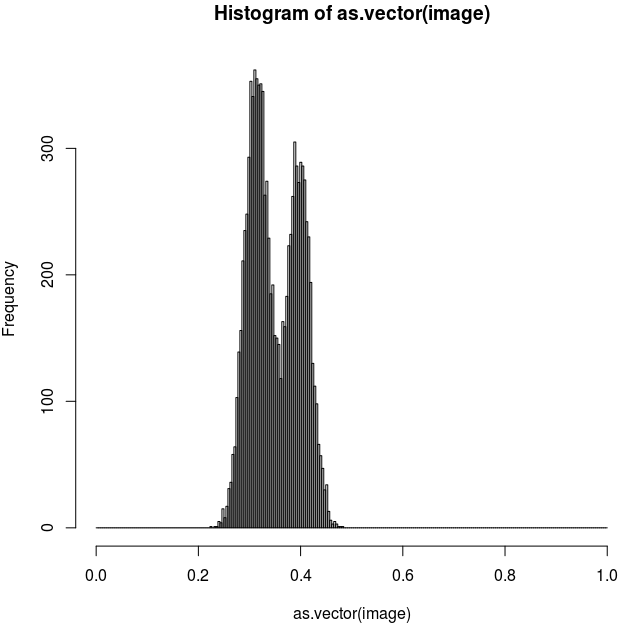
\includegraphics[scale=0.3]{image/histo.png}
\end{figure}

Les valeurs de l'histogramme représentent le nombre de pixels pour un niveau de gris donné. Les valeurs données (les seuils) représentent le seuil de coupure de notre histogramme, c'est un pourcentage. Notre histogramme va de 0 à 255 où de 0 à 1. 0.35, définit le seuil où on sépare l'histogramme.\\

\begin{lstlisting}
binaire1 <- (image - 0.35)>= 0
binaire2 <- (image - 0.36)>= 0
binaire3 <- (image - 0.37)>= 0
display(binaire1, "binaire 1")
display(binaire2, "binaire 2")
display(binaire3, "binaire 3")
nbins <- 256
h <- hist (as.vector (image), breaks = seq (0, 1, 1 / nbins))
\end{lstlisting}

\begin{figure}[!ht]
	\center
	
\includegraphics[scale=1]{image/binaire1.png}
	
\includegraphics[scale=1]{image/binaire2.png}
	
\includegraphics[scale=1]{image/binaire3.png}
\end{figure}

À la vue de nos binarisations on observe que aucune de ces images permet une parfaite binarisation. Soit la partie noir s'approche de la perfection, soit c'est la partie blanche.

\newpage

\section*{Question 2}

\begin{figure}[!ht]
	\center
	
\includegraphics[scale=1]{image/2classes_100_100_8bits_omega1.png}
	\hspace{6em}
	
\includegraphics[scale=1]{image/2classes_100_100_8bits_omega2.png}
\end{figure}
\begin{figure}[!ht]
	\center
	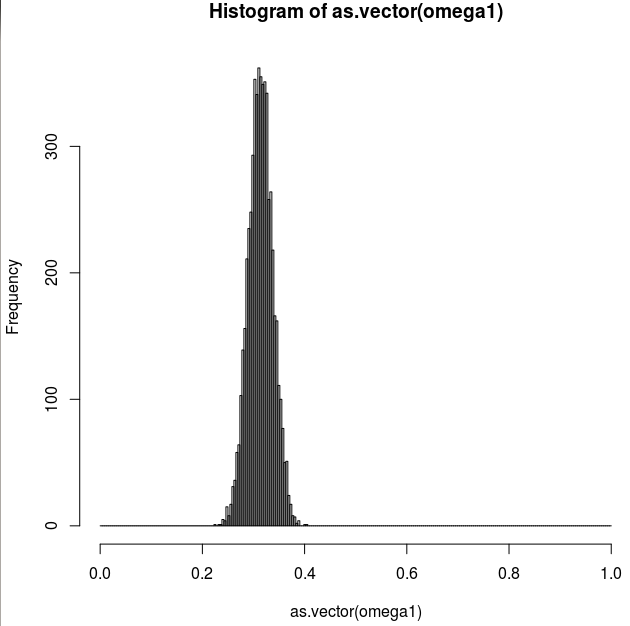
\includegraphics[scale=0.3]{image/q21.png}
	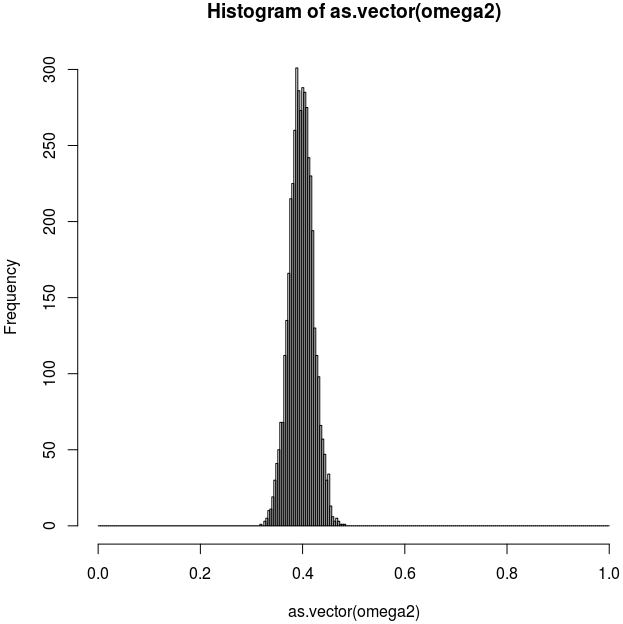
\includegraphics[scale=0.3]{image/q22.png}
\end{figure}

\begin{lstlisting}
h1 <- hist (as.vector (omega1), breaks = seq (0, 1, 1 / nbins))
h2 <- hist (as.vector (omega2), breaks = seq (0, 1, 1 / nbins))
N = sum(h$counts) # Nb de pixels total de l'image
N1 = sum(h1$counts) # Nb de pixels de la classe omega 1
N2 = sum(h2$counts) # Nb de pixels de la classe omega 2
Pomega1 = N1/N
Pomega2 = N2/N
\end{lstlisting}


La probabilité pour un pixel d'être dans une classe particulière est :

\begin{itemize}
	\item	P($\omega$1) = 0.56
	\item 	P($\omega$2) = 0.44
\end{itemize}

\newpage


\section*{Question 3}

\begin{lstlisting}
ndg <- 89
PIconditionnelle <- h$counts[ndg]/N
PO1conditionnelle <- h1$counts[ndg]/N1
PO2conditionnelle <- h2$counts[ndg]/N2
\end{lstlisting}

Nombre de pixels ayant le niveau de gris 89 dans chaque image sont :

\begin{itemize}
	\item I = 192
	\item $\omega$1 = 162
	\item $\omega$2 = 30
\end{itemize}

Les probabilitées d'avoir le niveau de gris 89 dans chaque image sont :

\begin{itemize}
	\item P(89/I) = 0.0192
	\item P(89/$\omega$1) = 0.0289
	\item P(89/$\omega$2) = 0.0068
\end{itemize}

\newpage

\section*{Question 4}

\begin{lstlisting}
# Seuillage automatique - Proba d'erreur
somme1 = 0:255
somme2 = 0:255
erreur = 0:255
# recherche du minimum
minimum_erreur = 1;
seuil_minimum_erreur = 0;

for (X in 1:255) {
  somme1[X+1]=sum(h1$density[(X+1):256])/sum(h1$density[1:256])
  somme1[X+1]=somme1[X+1]*Pomega1

  somme2[X+1]=sum(h2$density[1:(X+1)])/sum(h2$density[1:256])
  somme2[X+1]=somme2[X+1]*Pomega2
  
  erreur[X+1] = somme1[X+1] + somme2[X+1]
# seuil corrrespondant a l'erreur minimale
  if (erreur[X+1] < minimum_erreur ) 
    seuil_minimum_erreur = X
  if (erreur[X+1] < minimum_erreur ) 
    minimum_erreur = erreur[X+1]
}

#seuillage de l'image
seuil_auto_img <- (image - seuil_minimum_erreur/255)>= 0##
display(seuil_auto_img)
\end{lstlisting}

On trouves un seuil optimal de 92.
Le taux d'erreur de classification est de 0.0471
Voici l'image obtenue:

\begin{figure}[!ht]
	\center
	
\includegraphics[scale=1]{image/image_seuil_auto.png}
\end{figure}

\newpage

\section*{Question 5}

Pour cette question nous avons appliqué tout ce qui a été vu précédemment. 
Concernant le code nous avons réutilisé l'intégralité des questions précédentes et changé le nom des images.

\begin{figure}[!ht]
	\center
	
\includegraphics[scale=2]{image/zero_traite.png}
\end{figure}



\section*{Conclusion}

En conclusion on obtient une binarisation avec un seuil déterminé automatiquement par des calculs de probabilité, solution optimale. On a pu distinguer toutes les zones avec des seuils différents pour chaque zone.

\end{document}
